\begin{frame}
  \frametitle{Web services}
  \begin{center}
    Web services
  \end{center}
\end{frame}

\begin{frame}
  \frametitle{Web services}
  \begin{center}
    what exactly are web services?
  \end{center}
\end{frame}

\begin{frame}
  \frametitle{Web services}
  \begin{center}
    API for web applications
  \end{center}
\end{frame}

\begin{frame}
  \frametitle{Web services}
  \begin{itemize}
  \item weather
  \item sport results
  \item stock market
  \item \alert{some more serious examples}
  \end{itemize}
\end{frame}

\begin{frame}
  \frametitle{Web services}
  \begin{center}
    a bit of history
  \end{center}
\end{frame}

\begin{frame}
  \frametitle{Web services}
  \begin{center}
    Remote Procedure Call
  \end{center}
\end{frame}

\begin{frame}
  \frametitle{Web services}
  \begin{center}
    XML-RPC
  \end{center}
\end{frame}

\begin{frame}
  \frametitle{Web services}
  \begin{center}
    uses XML over HTTP
  \end{center}
\end{frame}

\begin{frame}[fragile]
  \frametitle{Web services}
  \tiny \input{xml_rpc_request}
\end{frame}

\begin{frame}[fragile]
  \frametitle{Web services}
  \tiny \input{xml_rpc_response}
\end{frame}

\begin{frame}
  \frametitle{Web services}
  \begin{center}
    this evolved into
  \end{center}
\end{frame}

\begin{frame}
  \frametitle{Web services}
  \begin{center}
    SOAP
  \end{center}
\end{frame}

\begin{frame}
  \frametitle{Web services}
  \begin{center}
    \alert{Simple} Object Access Protocol
  \end{center}
\end{frame}

\begin{frame}
  \frametitle{Web services}
  \begin{center}
    this acronym was dropped with Version 1.2 of the standard
  \end{center}
\end{frame}

\begin{frame}
  \frametitle{Web services}
  \begin{itemize}
  \item it was confused with SOA
  \item it’s not that simple after all
  \end{itemize}
\end{frame}

\begin{frame}
  \frametitle{Web services}
  \begin{center}
    uses XML over HTTP
  \end{center}
\end{frame}

\begin{frame}[fragile]
  \frametitle{Web services}
  \tiny \input{soap_request}
\end{frame}

\begin{frame}[fragile]
  \frametitle{Web services}
  \tiny \input{soap_response}
\end{frame}

\begin{frame}
  \frametitle{Web services}
  \begin{center}
    services are defined using\\Web Services Description Language\\(WSDL)
  \end{center}
\end{frame}

\begin{frame}
  \frametitle{Web services}
  \begin{itemize}
  \item lets tools create client APIs
    \note{MS employee saying they made SOAP so complex, to be not
      human readable}
  \item client developers see methods with parameters
  \end{itemize}
\end{frame}


\begin{frame}[fragile]
  \frametitle{Web services}
  \tiny \input{wsdl_begin}
\end{frame}

\begin{frame}
  \frametitle{Web services}
  \begin{center}
    ... about 100 lines of XML later ...
  \end{center}
\end{frame}

\begin{frame}[fragile]
  \frametitle{Web services}
  \tiny \input{wsdl_end}
\end{frame}

\begin{frame}
  \frametitle{Web services}
  WS-* specifications
  \begin{itemize}
  \item WS-Addressing
  \item WS-Security
  \item WS-Trust
  \item WS-SecureConversation
  \item WS-ReliableMessaging
  \item WS-AtomicTransaction
  \item WS-Coordination
  \item WS-Policy
  \item WS-MetadataExchange
  \item ...
  \end{itemize}
\end{frame}

\begin{frame}[plain]
  \begin{changemargin}{-1cm}{-1cm}
    \begin{center}
      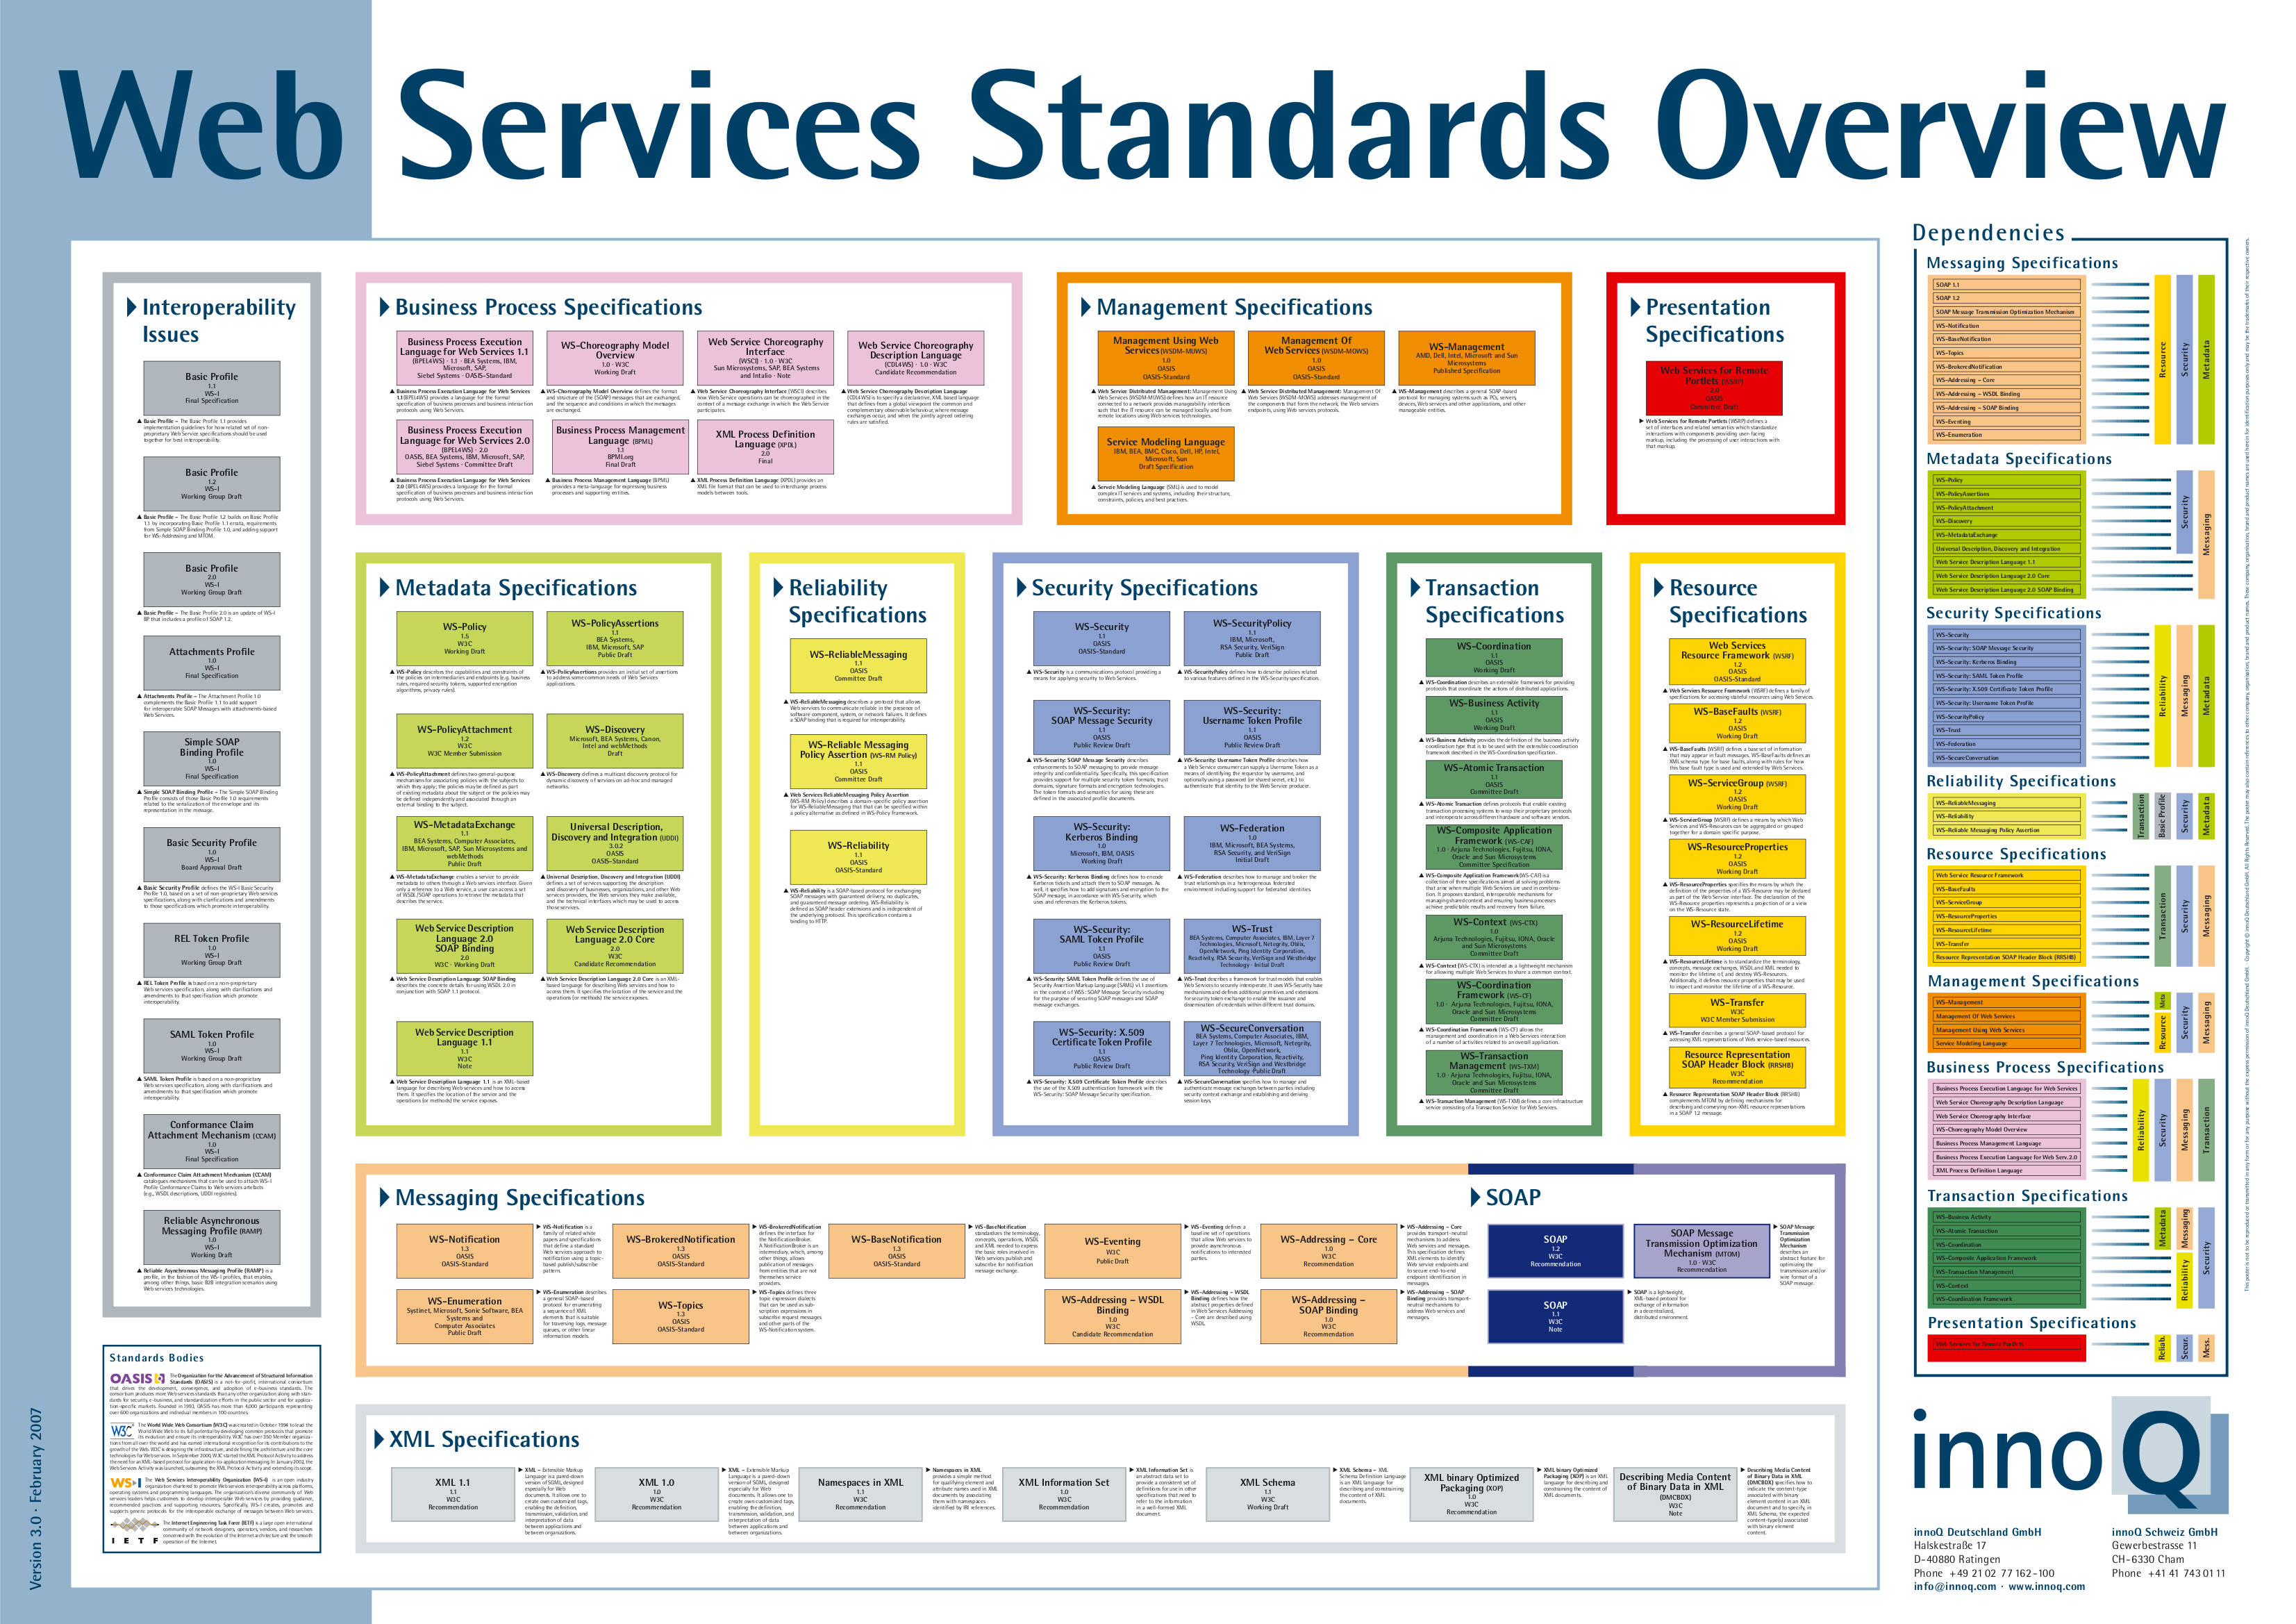
\includegraphics[width=\paperwidth, height=\paperheight, keepaspectratio]{images/WS-Standards-Poster.jpg}
    \end{center}
  \end{changemargin}
\end{frame}

\begin{frame}
  \frametitle{Web services}
  \begin{center}
    service oriented design
  \end{center}
\end{frame}

\begin{frame}
  \frametitle{Web services}
  \begin{itemize}
  \item UserManager
    \begin{itemize}
    \item createUser(u:User)
    \item getUserDetails(id:ID)
    \end{itemize}
  \item StatusManager
    \begin{itemize}
    \item submitStatus(u\_id:ID, s:Status)
    \item getStatusDetails(u\_id:ID)
    \end{itemize}
  \end{itemize}
\end{frame}

\begin{frame}
  \frametitle{Web services}
  \begin{itemize}
  \item Pros
    \begin{itemize}
    \item it's a standard
    \item strong typing
    \item \alert{dopisac kolejne}
    \end{itemize}
  \item Cons
    \begin{itemize}
    \item complex
    \item strong typing
    \item \alert{dopisac kolejne}
    \end{itemize}
  \end{itemize}
\end{frame}

\begin{frame}
  \frametitle{Web services}
  \begin{center}
    not everyone needs enterprisey and complex web services
  \end{center}
\end{frame}

\begin{frame}
  \frametitle{Web services}
  \begin{center}
    you don't have to use SOAP
  \end{center}
\end{frame}

\begin{frame}
  \frametitle{Web services}
  \begin{center}
    others don't
  \end{center}
\end{frame}

\begin{frame}[plain]
  \begin{changemargin}{-1cm}{-1cm}
    \begin{center}
      
\includegraphics[width=\paperwidth, height=\paperheight, keepaspectratio]{images/dirty-harry.jpg}
    \end{center}
  \end{changemargin}
\end{frame}

\begin{frame}
  \frametitle{Web services}
  \begin{itemize}
  \item Amazon Web Services - provides both
    \begin{itemize}
    \item 20\% uses SOAP
    \item 80\% uses REST
    \end{itemize}
  \item Google Search API - deprecated SOAP in favor of REST
  \item Yahoo API - uses REST only
  \end{itemize}
\end{frame}
